% The workflow figure of paper.md: xelatex flow.tex
\documentclass[border=4pt]{standalone}
\usepackage{tikz}
\usetikzlibrary{positioning}
\begin{document}
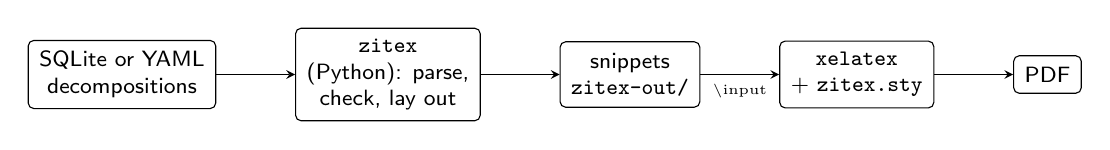
\begin{tikzpicture}[node distance=10mm, every node/.style={font=\footnotesize\sffamily},
    box/.style={draw, rounded corners=2pt, align=center, inner sep=4pt}, >=stealth]
  \node[box] (db) {SQLite or YAML\\decompositions};
  \node[box, right=of db] (py) {\texttt{zitex}\\(Python): parse,\\check, lay out};
  \node[box, right=of py] (snip) {snippets\\\texttt{zitex-out/}};
  \node[box, right=of snip] (xe) {\texttt{xelatex}\\+ \texttt{zitex.sty}};
  \node[box, right=of xe] (pdf) {PDF};
  \draw[->] (db) -- (py);
  \draw[->] (py) -- (snip);
  \draw[->] (snip) -- node[below, font=\tiny]{\textbackslash input} (xe);
  \draw[->] (xe) -- (pdf);
\end{tikzpicture}
\end{document}
